\chapter{Úvod}

V súčasnosti je čoraz častejšie zabezpečiť si svoj dom alebo byt aj inými technológiami ako sú mechanické zabezpečenie. To je často jednoduché prekonať a odradí len časť potenciálnych zlodejov. Rozšírením pre tento systém môže byť napríklad domáce zabezpečovacie zariadenie alebo presnejšie elektronický zabezpečovací systém. Vďaka tomuto systému je možné identifikovať prítomnosť zlodeja aj po prekonaní mechanických systémov. Takéto zariadenia sú stále dostupnejšie a inteligentnejšie. Pri každom príchode a odchode z domu je však nutné tento systém zapnúť, respektíve vypnúť. To môže byť často otravné. Nutnosť stále zadávať kód a zároveň nezabudnúť toto zariadenie aktivovať. Preto som sa rozhodol zamyslieť sa nad otázkou: Čo ak by zariadenie dokázalo detekovať prítomnosť majiteľa pri priblížení k objektu a detekovať jeho odchod?

Cieľom práce je vytvoriť zabezpečovacie zariadenie, ktoré pomocou Bluetooth dokáže detekovať prítomnosť majiteľa~-~jeho telefónu, hodiniek a podobne. Použitie Bluetooth je vhodné hlavne vďaka množstvu zariadení, ktoré ho podporujú. Ide hlavne o nositeľné zariadenia a zariadenia, ktoré majú ľudia stále pri sebe.
Súčasťou práce bude zároveň aj vytvoriť mobilnú aplikáciu, ktorá bude slúžiť na nastavenie systému a jeho správu. Podporovať by mala najrozšírenejšie mobilné operačné systémy ako Android a iOS.

\chapter{Zabezpečovacie systémy}

Vo všeobecnosti sa medzi k zabezpečovacej technike radí viacero systémov zabezpečovania. Patria sem napríklad mechanické zábranné systémy (zámok, plot a pod.), elektronické zabezpečovacie systémy (EZS), elektronická požiarna signalizácia, systémy priemyselnej televízie (CCTV) a IP kamerové systémy. V tejto práci sa ďalej zameriam na elektronické zabezpečovacie systémy, ich využitie v domoch a bytoch. Ďalšie zabezpečovacie systémy sú spomenuté len stručne ako možné rozšírenia systému, keďže moderné zabezpečovacie systémy sa často spájajú do jedného systému, ktorý dokáže ochrániť domácnosť nie len pred zlodejmi ale aj prírodnými živlami.

\section{Elektronické zabezpečovacie systémy}

Elektronický zabezpečovací systém je poplachový systém pre detekciu a indikáciu prítomnosti, vstupu alebo pokusu o vstup narušiteľa do stráženého objektu. Rozdeľujeme ich podľa stupňa zabezpečenia do 4 kategórií, viď tabuľka \ref{tab:stupenzabezpecenia}.
\begin{table}[ht]
    \centering
    \renewcommand{\arraystretch}{1.5}
    \begin{tabular}{|c|c|p{8cm}|}
        \hline
        \textbf{Stupeň} & \textbf{Miera rizika} & \textbf{Predpokladaný typ narušiteľa}\\ \hline
        1& nízke & narušiteľ má malú znalosť EZS; obmedzený sortiment ľahko dostupných nástrojov\\ \hline
        2 & nízke až stredné &narušiteľ má určité znalosti o EZS; obmedzený sortiment základných prenosných prístrojov (napríklad multimeter)\\ \hline
        3 & stredné až vysoké & narušiteľ je oboznámený s EZS; úplný sortiment prenosných prístrojov a elektronických zariadení \\ \hline
        4 & vysoké & narušiteľ je schopný alebo má možnosť spracovať podrobný plán vniknutia; kompletný sortiment zariadení vrátane prostriedkov pre náhradu rozhodujúcich prvkov EZS\\ \hline
    \end{tabular}
    \caption{Stupne zabezpečenia\cite{csn-en-50131-1}\cite{Krecek}}
    \label{tab:stupenzabezpecenia}
\end{table}

Elektronické zabezpečovacie systémy sa vo všeobecnosti skladajú z rôznych prvkov. Sem patria prvky:\cite{velas_ezs}
\begin{itemize}
    \item plášťovej ochrany
    \item tiesňovej ochrany - verejné alebo skryté
    \item ovládacie zariadenia
    \item ústredne EZS
    \item signalizačné (výstražné) zariadenia - siréna, maják
    \item priestorovej ochrany
    \item predmetovej ochrany - napríklad na ochranu zavesených predmetov ako obrazy
    \item vonkajšej obvodovej ochrany
\end{itemize}
Podľa normy ČSN~EN~50131-1 musí EZS obsahovať:
\begin{itemize}
    \item ústredňu, 
    \item jeden alebo viac detektorov,
    \item jedno alebo viac signalizačných zariadení prípadne poplachových prenosných systémov,
    \item jedno alebo viac napájacích zariadení. 
\end{itemize}

Všetky komponenty EZS musia podľa normy ČSN~EN~50131-1 zaisťovať detekciu sabotáže. Teda musia obsahovať prostriedky k zamedzeniu prístupu k vnútorným súčiastkam, normálny prístup musí vyžadovať využitie vhodného nástroja. Prístup k prostriedkom určeným k orientácii zorného poľa detektoru nesmie byť prístupný neoprávneným osobám.\cite{csn-en-50131-1}

\subsection{Ústredňa EZS}

Je zariadenie určené k príjmu a vyhodnocovaniu výstupných elektrických signálov čidiel alebo tiesňových hlásičov a k vytvoreniu signálu o narušení. V prípade drôtových ústrední slúži zároveň aj ako zdroj napájania pre senzory. Medzi jej ďalšie funkcie patrí diagnostika systému a uvedenie systému do stavu stráženia alebo do stavu pokoja. Vstupom do ústredne sú vstupné vyhodnocovacie obvody, ktoré vyhodnocujú prijaté informácie zo senzorov. Zároveň do vstupov môžeme zaradiť aj ovládacie prvky systému. Výstupom sú indikačné zariadenia pre optickú a akustickú signalizáciu. Ústredňa môže byť doplnená aj o výstup telefónneho voliča, pripojenie na internet pre identifikovanie poplachu aj v prípade poškodenia indikačných zariadení alebo použitia takzvaného tichého poplachu, teda bez spustenia optickej a zvukovej signalizácie.

Ústredne je možné rozdeliť do štyroch základných skupín:
\begin{itemize}
    \item \textbf{slučkové} - pre každú poplachovú slučku má vlastný obvod, tie sú tvorené najčastejšie sériovým zapojením čidiel. Zmena odporu na slučke detekuje aktiváciu čidla alebo sabotáž na slučke. Systém má pomerne rozsiahlu káblovú sieť.
    \item \textbf{s priamou adresáciou čidiel} - funguje na princípe komunikácie na dátovej zbernici.Ústredňa generuje adresy jednotlivých čidiel a prijíma odozvy. káblová sieť je minimálna. Ústredňa dokáže identifikovať čidlo, ktoré spôsobilo poplach.
    \item \textbf{zmiešaného typu} - pracuje princípom dátovej komunikácie s koncentrátorom. Ten je pripojený na samotné čidla pomocou slučiek.
    \item \textbf{s bezdrôtovým prenosom signálu od čidiel} - ide o najnovší typ ústrední. Najčastejšie pracujú v pásme 433~MHz s výkonom okolo 10~mW. Vlastný dosah vo voľnom prostredí je 100~-~200~m. Čidla sú napájané z batérie.
    Podľa druhu komunikácie medzi ústredňou a čidlami môže tieto systémy ďalej rozdeliť na:
    \begin{itemize}
        \item \textit{s jednosmernou komunikáciou} - jednoduchšie systémy, v čidle sa nachádza vysielač a v ústredni prijímač. Najčastejšie pracujú pomocou systému pravidelnej kontroly vysielaním kontrolných telegramov. Vďaka tejto kontrole dokáže ústredňa zistiť poruchu či poškodenie čidla. Problémom týchto systémov je, že v prípade zaznamenania pohybu odosielajú poplachovú správu aj v prípade, že sa systém nachádza v stave odstrážené, to zbytočne vyčerpáva energiu zdroja. To je spôsobené tým, že čidlá nemajú informáciu o stave systému. Zároveň sú náchylnejšie na rušenie signálu, pretože kmitočet a modulácia sú nemenné.
        \item \textit{s obojsmernou komunikáciou} - každý prvok systému je vybavený vysielačom aj prijímačom. Výhodou oproti systémom s jednosmernou komunikáciou je, že systémy v stave pokoja nevysielajú, pri zapínaní systému si ústredňa overí stav prvkov, pri rušení je možné automatické preladenie na voľný kanál.
    \end{itemize}
\end{itemize}

V súčasnosti medzi najpoužívanejšie patria bezdrôtové systémy. Výhodou je hlavne jednoduchá inštalácia, ľahké rozšírenie systému o ďalšie senzory, flexibilita systému napríklad pri zmene rozostavenia nábytku a podobne. Tento spôsob komunikácie však prináša aj mnoho problémov, ktoré je potrebné riešiť. Jednou z nevýhod je napríklad nebezpečie rušenia komunikácie. To môže viesť k vzniku falošného poplachu, či strate spojenia. Samozrejmou požiadavkou je aj kódovanie komunikácie medzi prvkami systému. To znemožňuje skreslenie prenosu a zabraňuje neoprávnenému preniknutiu do systému.\cite{Krecek}

\subsubsection{Napájanie ústredne}

Keďže EZS musí fungovať aj v prípade výpadku elektrickej energie, musí byť napájací zdroj zálohovaný náhradným zdrojom napätia. Systém je teda okrem základného zdroja, ktorý slúži na trvalé napájanie EZS, vybavený aj náhradným napájacím zdrojom. Jeho kapacita sa líši podľa stupňa zabezpečenia (viď tabuľka \ref{tab:stupenzabezpecenia}) a je definovaná v norme ČSN~EN~50131-1.

\subsubsection{Zóny stráženia}

Podľa reakcie ústredne na výstupný signál z detektoru rozlišujeme rôzne typy slučiek, resp. zón. Medzi základné radíme:
\begin{itemize}
    \item \textbf{okamžitá slučka} - v pohotovostnom režime ústredňa nereaguje, v režime stráženia spôsobuje okamžite vyhlásenie poplachu. Do slučky sa pridávajú detektory kde sa nepredpokladá pohyb užívateľov počas ochrany objektu.
    \item \textbf{oneskorená slučka} - v pohotovostnom režime ústredňa nereaguje, v režime stráženia ústredňa vyhlási poplach až po presne stanovenom čase. Do oneskorených slučiek sú zapojené senzory, ktoré sa nachádzajú pri ovládacích prvkoch EZS (pri vstupe do objektu).
    \item \textbf{trvalá slučka} - ústredňa reaguje na narušenie okamžitým poplachom v stave stráženia aj v pohotovostnom režime.
\end{itemize}
Tieto základné typy môžu byť prípadne modifikované a rozšírené o ďalšie.\cite{velas_ezs}

\subsection{Detektory}

Detektor alebo čidlo EZS je zariadenie reagujúce na narušenie stráženého objektu vytvorením určitého výstupného poplachového signálu. Časť detektoru, ktorá sníma zmenu stavu nazývame senzor. Poznáme rôzne druhy detektorov. Podľa typu napájania ich môžeme rozdeliť na nenapájané a napájané, podľa druhu zabezpečenia na priestorové a smerové.

\subsubsection{Magnetický kontakt}

Je určený na stráženie stavebných otvorov ako sú okná, dvere, rolety a pod. Tvorí ho vždy dvojica dielov - jazýčkový kontakt a permanentný magnet. Jazýčkový kontakt je tvorený zatavenou sklenenou rúrkou, naplnenou ochrannou atmosférou. V nej sú umiestnené dva feromagnetické kontakty. Magnet sa montuje na pohyblivú časť okna (dverí) a jazýčkový kontakt na rám. V prípade, že sa magnet priblíži k jazýčkovému kontaktu, kontakty sa spoja viď obrázok \ref{fig:magnetickykontakt}. V prípade, že sa magnet vzdiali kontakty sa znova rozopnú. Magnetický kontakt môže byť zabudovaný aj priamo do rámu dverí alebo okna, to umožňuje skrytú montáž.\cite{velas_ezs}

\begin{figure}[hbt]
    \centering
    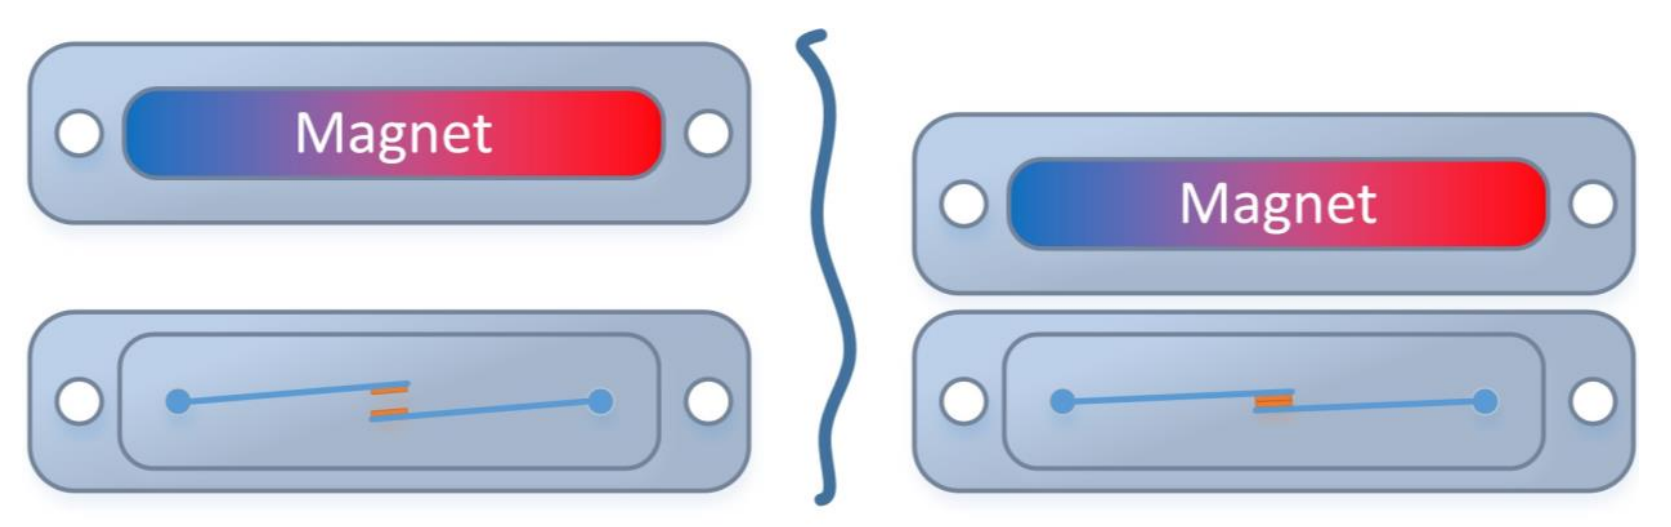
\includegraphics[width=\linewidth]{obrazky-figures/magnetickykontakt.png}
    \caption{Princíp činnosti magnetického kontaktu\cite{magnetickykontakt}}
    \label{fig:magnetickykontakt}
\end{figure}

\subsubsection{Detektory rozbitia skla}

Keďže najjednoduchším spôsobom ako preniknúť do stráženého objektu je práve cez rozbité okno je dôležité myslieť na ich ochranu. Existuje hneď niekoľko spôsobov ako detekovať rozbitie skla:
\begin{itemize}
    \item \textit{poplachové fólie} - pracujú na princípe vodivých pásikov alebo plôch zaliatych vo vnútri fólie. Poplach je vyvolaný prerušením vodivého pásika. Nalepujú sa na sklenené výplne dverí, okien a výkladov.
    \item \textit{kontaktné snímače} - pracujú na princípe uzavretého elektrického obvodu. Rozbitím skla sa naruší a vyvolá tak poplach. Nedostatkom je nízka odolnosť voči vyrazeniu skla.
    \item \textit{piezoelektrické snímače} - vyhodnocujú otrasy na skle, ktoré vznikajú pri rozbití, rezaní skla. Umiestňujú sa do rohu skla a majú dosah 1,5 až 3 m.
    \item \textit{akustické detektory rozbitia skla} - detekujú zvuk rozbitia skla pomocou mikrofónu. Majú dosah až 10 m od stráženého skla. Sú náchylnejšie na falošné poplachy, ktoré môže vyvolať zvoniaci telefón, rozbitie skla vonku či brzdenie električky.
\end{itemize}

\subsubsection{Pasívne infračervené detektory}

Pasívne infračervené detektory (PIR – Passive Infrared Receiver) snímajú zmeny v infračervenom pásme elektromagnetického vlnenia vo svojom okolí, na ich základe následne vyhodnocujú narušenie. Využíva sa pyroelektrický senzor, ktorý reaguje na pohybujúce sa teleso s teplotou odlišnou od teploty okolia. Ten je doplnený o optický systém, ktorý má funkciu zosilnenia signálu a zvýšenie citlivosti senzora. Využívajú sa Fresnelové šošovky alebo často sústava lomených zrkadiel napríklad tzv. čierne zrkadlo, ktoré neodráža viditeľne svetlo, ale naopak dobre odráža žiarenie vygenerované ľudským telom. PIR detektor je najcitlivejší na pohyb kolmý na optickú os detektora. Tieto detektory sú veľmi populárne najmä vďaka ich pomerne jednoduchej konštrukcii a nízkej cene. Ich výhodou je tiež, že dokážu detekovať prítomnosť človeka bez ožarovania elektromagnetickým vlnením, na ktoré môžu byť ľudia citlivý.\cite{velas_ezs}

V prípade EZS stupňa 3 a 4 (definované v tabuľke \ref{tab:stupenzabezpecenia}) musia byť detektory pohybu doplnené aj prostriedkami pre detekciu zakrytia (maskovania).\cite{csn-en-50131-1}

Na trhu sú dostupné detektory s rôznymi detekčnými charakteristikami (vejár, chodba, záves),
ktorých typ závisí od použitia danej šošovky. Ich detekčné charakteristiky môžeme vidieť na obrázkoch \ref{fig:pir-vejar}, \ref{fig:pir-zaclona}, \ref{fig:pir-chodba} a \ref{fig:pir-strop}. Kde v ľavej časti môžeme vidieť pohľad zhora a v pravej časti pohľad zo strany.

\begin{figure}[ht]
    \centering
    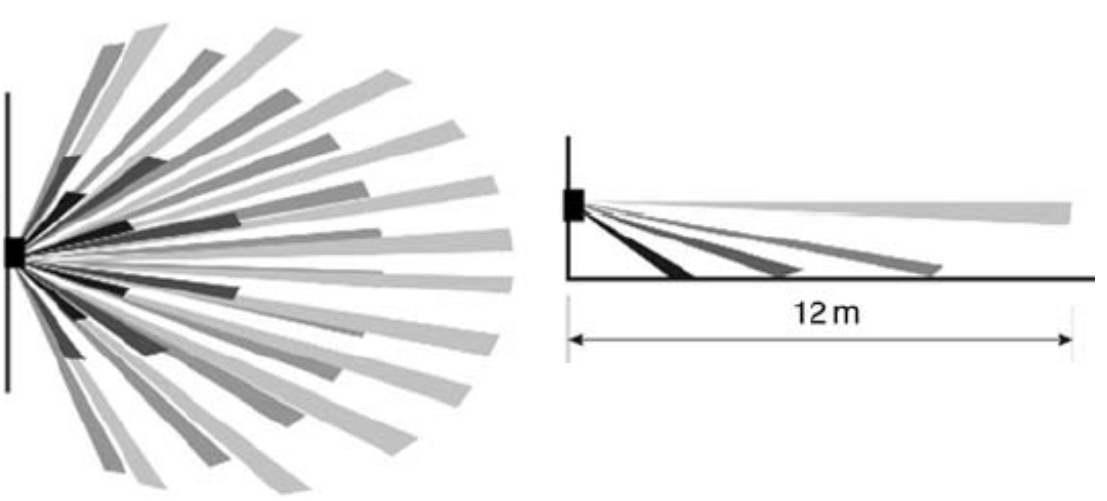
\includegraphics[width=0.75\linewidth]{obrazky-figures/PIR-vejar.png}
    \caption{Detekčná charakteristika PIR typu vejár\cite{PIR-vejar}}
    \label{fig:pir-vejar}
\end{figure}

\begin{figure}[ht]
    \centering
    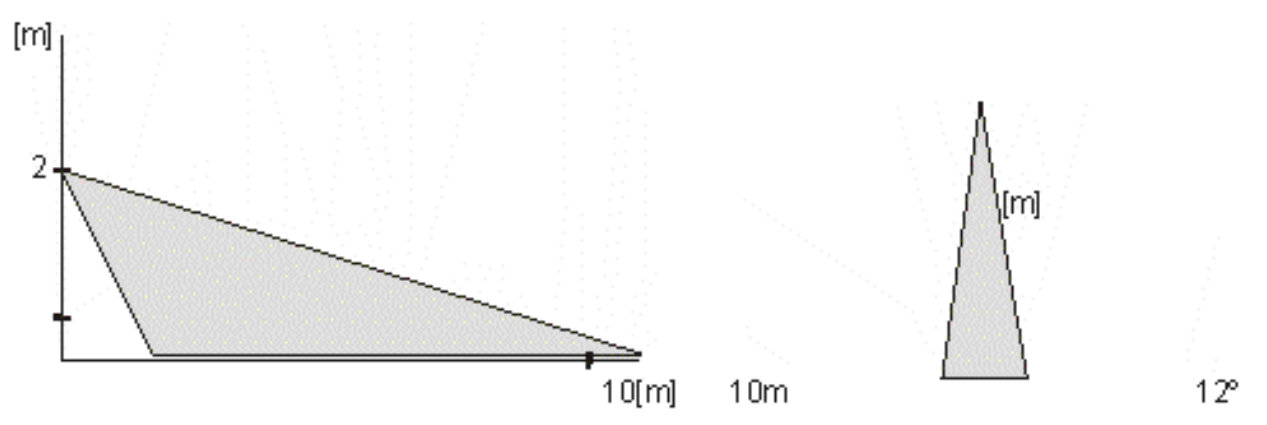
\includegraphics[width=0.75\linewidth]{obrazky-figures/PIR-zaclona.png}
    \caption{Detekčná charakteristika PIR typu záclona\cite{velas_ezs}}
    \label{fig:pir-zaclona}
\end{figure}

\begin{figure}[ht]
    \centering
    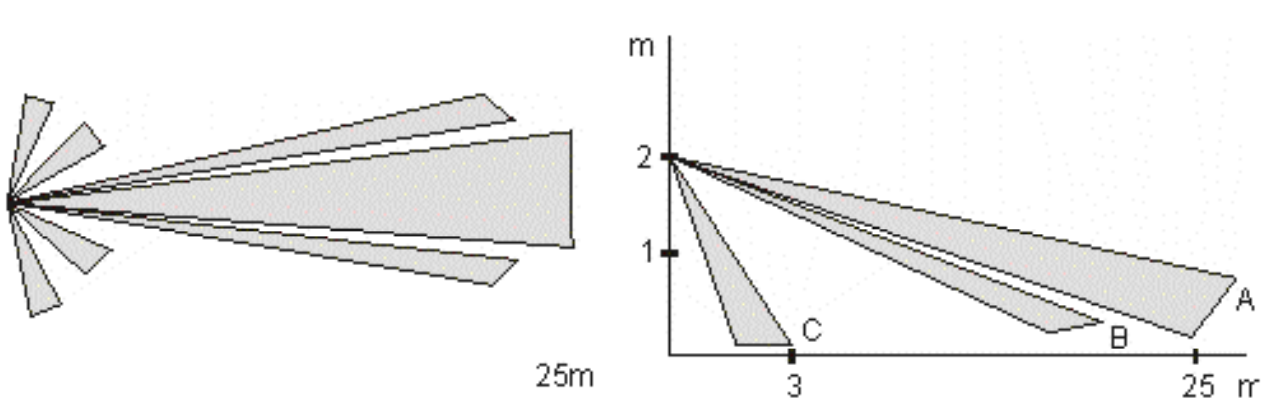
\includegraphics[width=0.75\linewidth]{obrazky-figures/PIR-chodba.png}
    \caption{Detekčná charakteristika PIR typu chodba\cite{velas_ezs}}
    \label{fig:pir-chodba}
\end{figure}

\begin{figure}[ht]
    \centering
    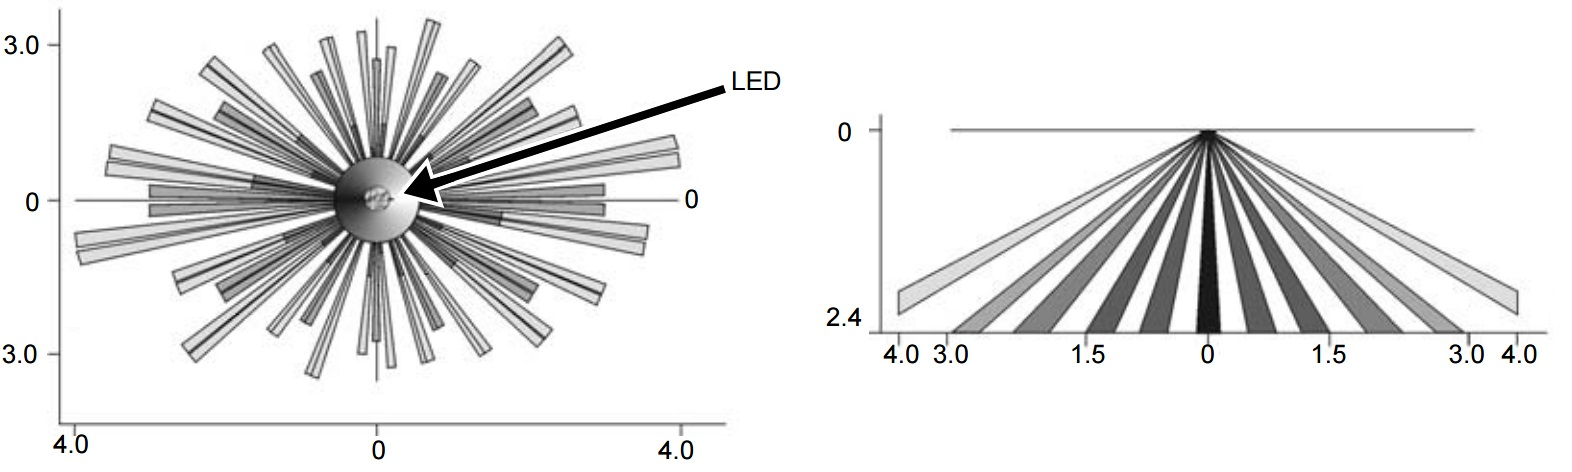
\includegraphics[width=0.75\linewidth]{obrazky-figures/PIR-strop.jpg}
    \caption{Detekčná charakteristika stropného PIR senzora\cite{PIR-strop}}
    \label{fig:pir-strop}
\end{figure}

\subsubsection{Ultrazvukové detektory}

Patria medzi aktívne prvky, teda do priestoru vysielajú energiu. Vysielač vysiela vlnenie konštantnej frekvencie nad pásmom počuteľného zvuku. Následne prijímač prijíma odrazený zvuk a vyhodnocuje fázy, ktoré vznikajú pri pohybe telesa v chránenom priestore. Jedná v podstate o aplikáciu Dopplerovho javu v pásme ultrazvuku. Na ultrazvuk môžu byť citlivé zvieratá (pes, netopier a pod.), ktoré tento zvuk môžu počuť. Dosah detektoru je približne 10 m. Ich citlivosť sa môže znížiť v prítomnosti materiálov, ktoré pohlcujú zvuk ako koberce, penové materiály a podobne.\cite{Krecek}

\subsubsection{Mikrovlnné detektory}

Vychádzajú z rovnakého princípu ako ultrazvukové detektory, pracujú však vo frekvenčnom pásme elektromagnetického vlnenia. Taktiež patria medzi aktívne prvky. Ich typický dosah je 15 až 30m. Na rozdiel od ultrazvukových a PIR senzorov sú citlivé na rušenie z okolia, preto je pravdepodobnosť vzniku falošného poplachu vyššia.\cite{velas_ezs}

\subsubsection{Duálne detektory}

Ide o spojenie PIR a ultrazvukového, prípadne mikrovlnného detektoru. Myšlienka za spojením je že, je malá pravdepodobnosť súčasného vzniku javov, ktoré by mohli vyvolať falošný poplach pri viacerých čidlách pracujúcich na rozdielnych fyzikálnych princípoch. Zároveň zvyšujú odolnosť voči poruchám. Detektory často umožňujú dve nastavenia - poplach sa spustí pri reakcii oboch čidiel alebo na vyvolanie poplachu stačí ľubovoľný detektor.\cite{velas_ezs}

\subsection{Overovanie spojenia}

Integrita spojenia senzorov s ústredňou musí byť pravidelne kontrolovaná v intervaloch špecifikovaných v tabuľke \ref{tab:interval_overenia}. Stupňom rozumieme stupeň zabezpečenia definovaný v tabuľke \ref{tab:stupenzabezpecenia} a jednotlivé časy sú maximálne prípustné intervaly medzi signálmi alebo správami komunikácie. V prípade, že komunikácia nie je v tomto čase overená, systém by mať vyvolať oznámenie o poruche, prípadne o sabotáži. Zároveň systém nesmie byť prepnutý do stavu stráženia, ak nebola komunikácia overená v intervale podľa tabuľky \ref{tab:interval_overenia}.

\begin{table}[ht]
    \centering
    \renewcommand{\arraystretch}{1.5}
    \begin{tabular}{|c|c|c|c|c|}
        \hline
         & Stupeň 1 & Stupeň 2 & Stupeň 3 & Stupeň 4 \\ \hline
        Periodická komunikácia & 240 min & 120 min & 100 s & 10 s \\ \hline
        Nastavovanie stavu stráženia & 60 min & 20 min & 60 s & 10 s\\ \hline
    \end{tabular}
    \caption{Intervaly overovania\cite{csn-en-50131-1}}
    \label{tab:interval_overenia}
\end{table}



\subsection{Ovládacie a indikačné zariadenia}

Ovládacie prvky slúžia na uvedenie systému do stavu stráženia alebo do stavu pokoja. Zároveň slúžia aj na zadávanie užívateľských kódov pre ovládanie systému, odstavenie poplachu, základnú správu systému.
\begin{itemize}
    \item \textbf{blokovací zámok} - kombinuje mechanické zabezpečenie vstupných dverí s ovládaním EZS. Pri odomknutí dverí sa systém automaticky uvedie do stavu odstrážené. Zároveň pri zamykaní sa systém uvedie do stavu zabezpečené. Zámok je pritom možné uzamknúť len ak je EZS v normálnom stave. Použitie je prirodzené a jednoduché. Ide o jeden z najnákladnejších spôsobov ovládania systému.
    \item \textbf{spínací zámok} - podobný blokovaciemu zámku, neobsahuje systém blokovania uzamknutia dverí v prípade poruchy či chyby obsluhy (napríklad otvorené okno)
    \item \textbf{kódové klávesnice} - je nutné aby elektronika klávesnice bola umiestnená v strážených priestoroch. Prináša nevýhodu, že užívateľ si musí zapamätať kód. Ten je však potrebné pravidelne meniť.
    \item \textbf{ovládanie kartou} - výhodou je multifunkčnosť karty a teda možnosť využiť ju na ďalšie použitie ako obedy, dochádzkový systém, parkovanie a podobne. Nevýhodou je prenosnosť karty, prípadne možnosť jej skopírovania.
    \item \textbf{diaľkové ovládanie} - musí byť chránené vhodným kódom, aby sa nedal zachytiť jeho signál a vyrobiť kópia. Môže byť doplnené aj o ďalšie funkcie ako spustenie tiesňového hlásenia a pod.\cite{velas_ezs}
\end{itemize}

Indikačné prvky informujú o stave systému napríklad pomocou LED diódy, akustickej, vizuálnej signalizácie, prípadne ich kombináciou. Medzi najbežnejšie hlásenia patria:
\begin{itemize}
    \item stav pokoja/stráženia
    \item uvádzanie do stavu stráženia
    \item hlásenie poruchy
    \item poplach
\end{itemize}

Akustické výstražné zariadenie musí byť v prevádzke aspoň 90 sekúnd pričom maximálna doba jeho činnosti nesmie prekročiť 15 minút.\cite{csn-en-50131-1}

Systém môže byť doplnený o ďalšie doplnkové zariadenia, ktoré slúžia na komunikáciu s pultom centrálnej ochrany alebo na komunikáciu s majiteľom.\cite{Krecek}

\section{Elektrická požiarna signalizácia}

Medzi hlavné ciele elektrickej požiarnej signalizácie(EPS) patrí rýchle a spoľahlivé určenie požiaru už v jeho počiatku, prípadne sú tieto systémy schopné začať tento požiar likvidovať, privolať pomoc a podobne. Požiar sa signalizuje opticky a akusticky.

Tieto systémy sú podobne ako EZS zložené z ústredne, hlásičov požiaru a ďalších doplňujúcich zariadení. Požiarne hlásiče môžu byť buď manuálne (tlačidlové) alebo automatické.
Automatické požiarne hlásiče môžeme rozdeliť na:
\begin{itemize}
    \item teplotné hlásiče
    \item ionizačné hlásiče dymu
    \item optické hlásiče dymu
    \item multisenzorové s využitím plynovej detekcie
    \item optické hlásiče požiaru
    \item lineárny optický hlásič
    \item lineárny tepelný detektor
    \item aspiračný požiarny hlásič
    \item tlakový hlásič\cite{Krecek}
\end{itemize}

\section{Systémy priemyselnej televízie CCTV}

\section{IP-kamerové systény}

\chapter{Bluetooth Low Energy}

Bluetooth je technológia na bezdrôtovú komunikáciu medzi dvoma a viacerými zariadeniami. Má široké využitie od rôznych ovládačov, cez prehrávanie hudby až po prenos súborov medzi zariadeniami. Operuje v rovnakom frekvenčnom pásme ako technológia Wi-Fi - 2,4 GHz. Vďaka tomu môžu menšie zariadenia využívajúce obe technológie súčasne používať spoločnú anténu, to však prináša aj nevýhodu v podobe rušenia.

Bluetooth Low Energy (BLE) je navrhované pre nízko energetickú operáciu. Od Bluetooth v4.0 je súčasťou štandardu. Je primárne učené na výmenu kratších informácií nižšou rýchlosťou. Tento štandard je často využívaný pri zaradeniach napájaných z batérie, ako sú napríklad zariadenia Internetu vecí(IoT). Zariadenia s podporou tejto technológie sú označované často ako \textit{Bluetooth Smart}, respektíve \textit{Bluetooth Smart Ready} pre zariadenia spájajúce BLE a klasické Bluetooth.

\section{Porovnanie s klasickým Bluetooth}

Obe technológie využívajú rovnaké frekvenčné pásmo 2,402 - 2,480 GHz. Využívajú však rozdielny počet a rozostupy kanálov. BLE obsahuje 40 kanálov s rozostupom 2 MHz. Z toho sú 3 kanály určené na prenos informácií o zariadení tzv. \textit{advertising}, zvyšných 37 je určených na prenos dát. V prípade klasického Bluetooth je týchto kanálov 79 a s rozostupom 1 MHz. V závislosti na použitej fyzickej vrstve protokol BLE dosahuje rýchlosť až 2 Mb/s (Bluetooth v5.0) oproti tomu klasické Bluetooth dosahuje rýchlosť až 3 Mb/s.

BLE je v závislosti na použití 2 až 100 krát menej náročný na spotrebu energie.
\cite{bluetooth}

\section{Topológia}
Bluetooth Low Energy dokáže pracovať s tromi rôznymi topológiami siete:
\begin{itemize}
    \item \textbf{Point-to-point} - komunikácia medzi dvomi zariadeniami (1:1), je podporovaná ako pre BLE tak aj pre Bluetooth. Využíva sa napríklad na prehrávanie hudby. Táto topológia je vhodná pre rôzne typy zariadení. V prípade BLE sa táto topológia využíva napríklad pre fitnes zariadenia, merače tepu, periférie a príslušenstvo pre počítač.
    \item \textbf{Broadcast} - jedno zariadenie komunikuje s viacerými zariadeniami (1:M). Táto topológia je podporovaná len v BLE, využíva sa napríklad na lokalizáciu a navigáciu vo vnútri budovy.  
    \item \textbf{Mesh} - komunikácia viacerých zariadení (M:N), je podporovaná len pre BLE. Vďaka tejto topológii je možné vytvoriť veľkú sieť zariadení. Táto topológia je vhodná ak je potrebné spojiť desiatky, stovky či tisícky zariadení, ktoré potrebujú medzi sebou spoľahlivo a bezpečne komunikovať. Využitie má napríklad v monitorovaní alebo automatizácii.\cite{bluetooth}
\end{itemize}

\section{Architektúra} \label{sec:arch}
Bluetooth implementuje kompletnú architektúru od fyzickej komunikácie medzi zariadeniami až po komunikáciu s vlastnými aplikáciami, Bluetooth je teda takzvaný \textit{full protocol stack}. Kompletnú architektúru môžeme vidieť na obrázku \ref{fig:ble_stack}.

\begin{figure}[ht]
    \centering
    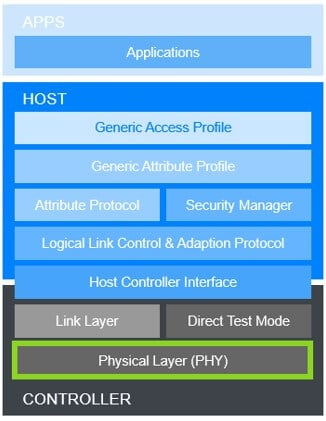
\includegraphics[scale=0.6]{obrazky-figures/bluetooth_le_protocol_stack.jpg}
    \caption{Architektúra BLE\cite{bluetooth}}
    \label{fig:ble_stack}
\end{figure}

\begin{itemize}
    \item \textbf{Physical Layer (PHY)} - fyzická vrstva, prenáša samotný analógový signál a transformuje ho na digitálny. Od Bluetooth v5.0 rozlišujeme 3 varianty PHY. Sú to:
    \begin{itemize}
        \item LE 1M - rýchlosť prenosu dát 1~Mb/s, pôvodná PHY definovaná v Bluetooth v4.0, chyby dokáže detekovať, ale nie opraviť
        \item LE 2M - rýchlosť 2~Mb/s, vzdialenosť prenosu je oproti LE 1M zmenšená na 80\%, chyby dokáže detekovať, ale nie opraviť
        \item LE Coded - dokáže teoreticky zvýšiť vzdialenosť prenosu dvoj až štvornásobne, a to pomocou redundancie dát v odosielanom pakete. Vďaka tomu zariadenie na druhej strane dokáže detekovať a opraviť chyby v dátach. Existujú dve varianty v závislosti na úrovni redundancie - S=2 a S=8, kde S udáva počet redundantných dát v odosielanom pakete. To ma však nepriaznivý vplyv na rýchlosť odosielania, ktorá je znížená na 500~Kb/s, resp. pre S=8 na 125~Kb/s. 
    \end{itemize}
    \item \textbf{Link Layer} - linková vrstva, jej úlohou je skenovanie, spravuje, vytvára spojenia
    \item \textbf{Direct Test Mode} - umožňuje testovanie fyzickej vrstvy
    \item \textbf{Host Controller Interface (HCI)} - sprostredkúva komunikáciu medzi vrstvami, môže využívať API alebo aj iné štandardné rozhrania ako USB, UART, SPI. 
    \item \textbf{Logical Link Control and Adaption protocol (L2CAP)} - zapuzdruje dáta pre ďalšie vrstvy
    \item \textbf{Attribute Protocol} - samotné zdieľané dáta
    \item \textbf{Security Manager} - zabezpečuje párovanie a distribúciu kľúčov
    \item \textbf{Generic Attribute Profile (GATT)}
    \item \textbf{Generic Access Profile (GAP)} - priama komunikácia s aplikáciou, zabezpečuje pripojenia na služby pre BLE zariadenie
    \cite{bluetooth}\cite{ble-arch}
\end{itemize}
Bližšie sa k GAP a GATT venujem v nasledujúcich podkapitolách \ref{sec:gap} a \ref{sec:gatt}.

\section{Rozsah pokrytia}

Rozsah pokrytia Bluetooth je závislý na viacerých faktoroch. Teoreticky je možné dosiahnuť vzdialenosť od metra až cez jeden kilometer. Bluetooth je navrhované na podporu rôznych rozsahov, konkrétna implementácia je ponechaná na vývojároch, aby si vybrali vhodné riešenie pre ich potreby. Jedným z faktorov je výber fyzickej vrstvy (PHY), kde rozdiely boli spomínané už v podkapitole \ref{sec:arch}. Ďalšími faktormi sú senzitivita prijímača, vysielací výkon, dosah antény alebo strata signálu po ceste, napríklad vďaka prekážkam a podobne.\cite{bluetooth}

\section{Generic Access Profile (GAP)}\label{sec:gap}

Ide o základný profil, ktorý implementujú všetky Bluetooth zariadenia. Definuje základne požiadavky zariadenia. Vyskytuje sa ako v klasickej (BR/EDR) verzii tak aj v Low Energy. Pre BLE definuje jednotlivé vrstvy architektúry, správanie a metódy pre vyhľadanie zariadenia, pripojenie k nemu, bezpečnosť a podobne.
Zároveň definuje 4 špecifické roly, pričom zariadenie môže podporovať viacero rolí súčasne. Každá z rolí je optimalizovaná je špecifické použitie. Sú to:
\begin{itemize}
    \item \textbf{Broadcaster} - vysielanie dát, nepodporuje spojenia
    \item \textbf{Observer} - prijímanie dát, komplementárny k Broadcaster, nepodporuje spojenia
    \item \textbf{Peripheral} - podporuje jedno spojenie, menej komplexné ako Central
    \item \textbf{Central} - podporuje niekoľko spojení\cite{bluetooth}
\end{itemize}

\section{Attribute Protocol}

Umožňuje čítať a zapisovať malé dáta na server. Každá hodnota, typicky pár bajtov, sa nazýva atribút (attribute). Tento protokol definuje pre každú hodnotu univerzálnu unikátnu identifikáciu~-~UUID. Tie môžu mať dĺžku 16, 32 alebo 128 bitov.
Protokol definuje dve roly~-~klient a server. Zariadenie dokáže zároveň fungovať ako server aj ako klient. Server ukladá dáta a akceptuje požiadavky, príkazy a potvrdenia od klienta. Taktiež odosiela odpovede a upozornenia pri výskyte špecifikovanej udalosti na serveri.\cite{bluetooth}

\subsection{Generic Attribute Profile (GATT)}\label{sec:gatt}

GATT definuje hierarchickú štruktúru dát. Je postavený na Attribute profile a definuje operácie nad dátami uloženými a zasielanými pomocou neho. taktiež špecifikuje formát dát, ktoré sa nachádzajú na serveri, sú formátované ako služby (services) a charakteristiky (characteristics). Jedna služba môže obsahovať niekoľko charakteristík. Služby môžu byť aj zanorené pričom zanorená služba existuje aj samostatne aj v rámci nadradenej služby. Charakteristiky obsahujú jednu hodnotu, jej vlastnosti a môžu obsahovať aj niekoľko deskriptorov, ktoré opisujú hodnotu. Na obrázku \ref{fig:gatt} je možné vidieť ako by napríklad mohla vyzerať hierarchia GATT.\cite{bluetooth}

\begin{figure}[ht]
    \centering
    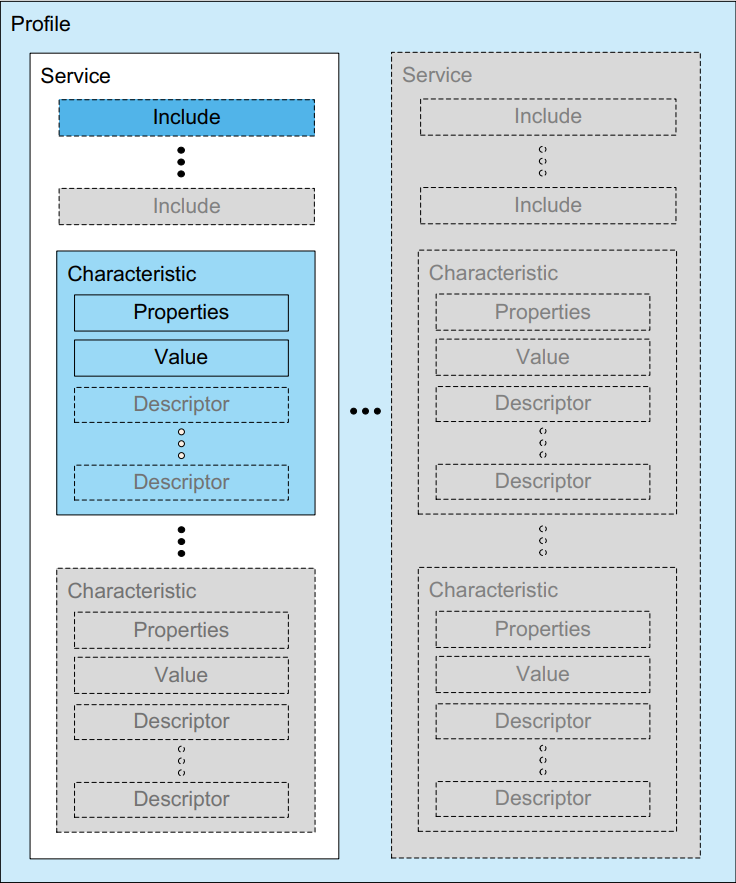
\includegraphics[scale=0.4]{obrazky-figures/gatt.png}
    \caption{Profilová hierarchia založená na GATT\cite{bluetooth}}
    \label{fig:gatt}
\end{figure}


\section{Párovanie zariadení}

Pri BLE môžeme rozlišovať dva spôsoby spojenia zariadení a výmeny kľúčov. V prípade, že ide o dočasné kľúče a krátkodobé tzv. \textit{párovanie} je spojenie len dočasné a je nutné pri každom párovaní vymeniť dočasné kľúče. V prípade viazania alebo presnejšie \textit{bonding} si zariadenia uložia dlhodobé kľúče do internej pamäte. Vďaka tomu dokážu šifrovať komunikáciu, overovať podpísané dáta a rozšifrovať náhodne generované adresy.
Proces viazania (bonding) zariadení môžeme rozdeliť na 3 fázy, tento proces môžeme pre názornosť lepšie pochopiť na obrázku \ref{fig:bonding}. V prípade párovania je postup rovnaký, ale končí sa fázou 2. Tieto fázy sú:
\begin{itemize}
    \item fáza 1 - výmena informácii o podporovaných vstupoch a výstupoch (potrebné pre zadanie alebo zobrazenie dočasného kľúča) , možnostiach zabezpečenia ako ochrana proti odchytávaniu komunikácie alebo tzv. \textit{Man-In-The-Middle} útoku. Nasleduje výmena párovacej informácie medzi zariadeniami. Okrem iného je v týchto paketoch znak definujúci, či sa jedná o párovania alebo následne aj bonding.
    \item fáza 2 - nasleduje výmena dočasných kľúčov pre šifrovanie komunikácie. Existuje niekoľko spôsobov výmeny týchto kľúčov. Časté je generovanie 6 miestneho kódu na jednej strane a prepísanie na druhej, porovnávanie kódov, jednoduché potvrdenie tlačidlom alebo využitie inej technológie na distribúciu kľúča (napr. NFC). Následne sa ešte overia kľúče. V prípade párovania nasleduje odosielanie samotných dát.
    \item fáza 3 - Táto časť komunikácie je už šifrovaná kľúčmi vygenerovanými vo fáze 2. Nasleduje generovanie a výmena dlhodobých kľúčov a výmena samotných dát. Pri ďalšom pripojení tento proces nie je potrebné opakovať.\cite{bluetooth}
\end{itemize}

\begin{figure}[ht]
    \centering
    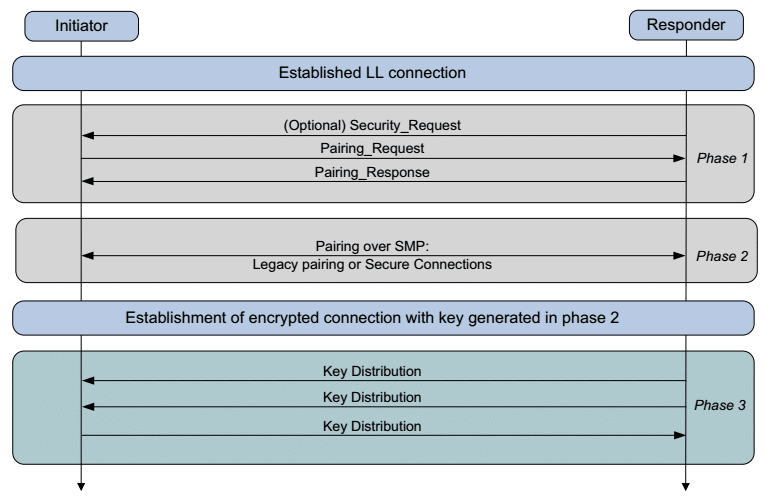
\includegraphics[width=0.75\linewidth]{obrazky-figures/pairing-flowchart.png}
    \caption{Bonding diagram komunikácie\cite{bluetooth}}
    \label{fig:bonding}
\end{figure}



\chapter{ESP32}

ESP32 je populárna séria systémov na čipe (SoC - System on chip) od spoločnosti Espressif Systems, ktorá vznikla v roku 2016. Je nasledovníkom známeho ESP2866. Ide o výkonnejší modul, ktorý má veľa ďalších vlastností ako podporu Bluetooth, viac GPIO pinov a podobne. V závislosti na variante existujú rôzne výkonné modely s rôznymi vlastnosťami.
Vďaka jeho pomerne nízkej cene a nízkej spotrebe je vhodný na automatizáciu domácnosti, v IoT zariadeniach, v medicíne, priemysle a podobne. Bol navrhnutý ako samostatne fungujúci mikrokontrolér s ohľadom na maximálny výkon s minimálnou spotrebou energie.

\section{Architektúra}

\begin{figure}[ht]
    \centering
    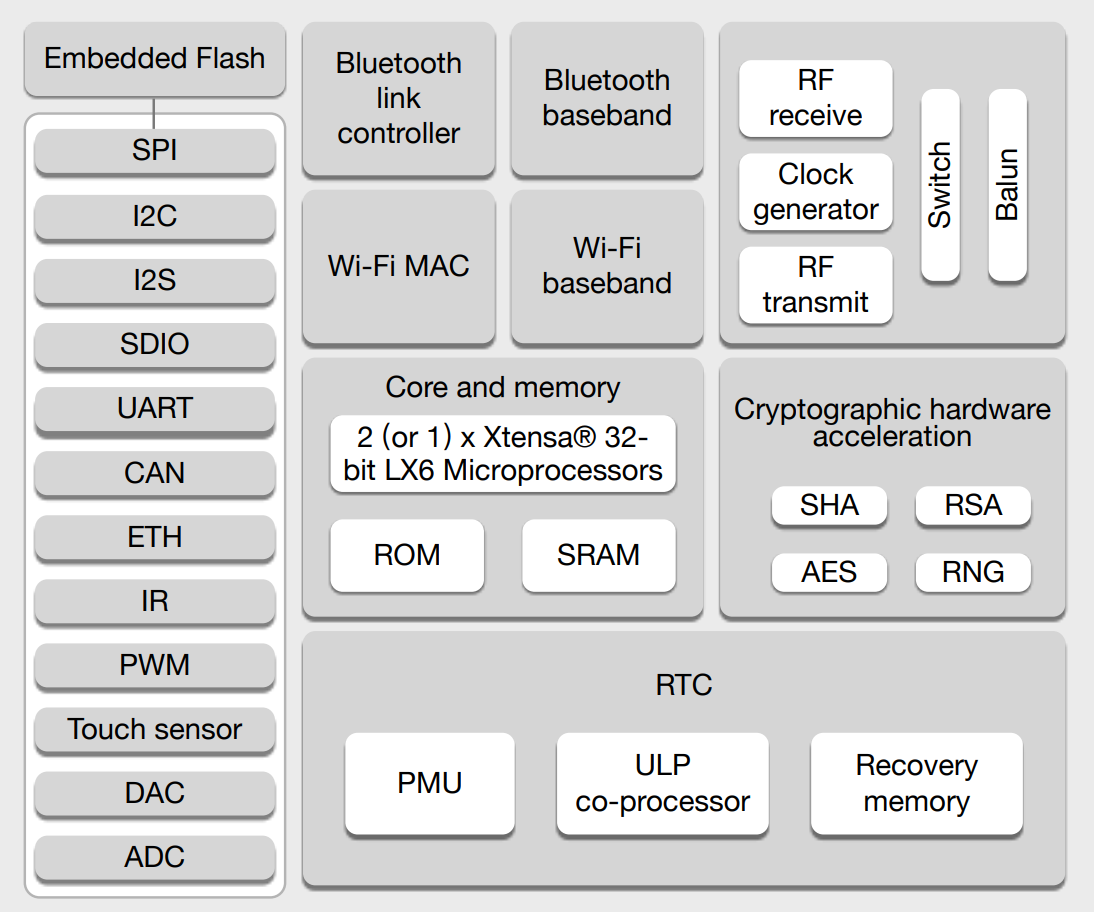
\includegraphics[scale=0.3]{obrazky-figures/esp32_diagram.png}
    \caption{Funkčný blokový diagram ESP32\cite{esp-datasheet}}
    \label{fig:esp_diagram}
\end{figure}

Jadrom ESP32 je 32-bitový procesor Xtensa s jedným alebo dvomi jadrami a frekvenciou až 240Mhz, ten je doplnený o 520~KB SRAM a 448~KB ROM. Zároveň na čipe môžeme nájsť podporu aj pre Wi-Fi 2,4~Ghz (802.11~b/g/n), Bluetooth v4.2 BR/EDR aj BLE (podľa aktuálnych informácií bol certifikovaný aj na v5.0\footnote{\url{https://www.espressif.com/en/news/BLE_5.0_Certification}}).
Čip má podporu aj pre hardvérovú akceleráciu šifrovania, množstvo rôznych periférií a 34 vstupno-výstupných portov (GPIO). Celý blokový diagram je znázornený na obrázku \ref{fig:esp_diagram}.\cite{esp-datasheet}


\section{Varianty}

ESP32 je dostupné v niekoľkých verziách. Tie môžeme v základe rozdeliť na SoC, moduly a vývojové dosky, viď obrázok \ref{fig:esp32_varianty}. Tie sa ďalej rozdeľujú napríklad podľa špecifikácií a dostupných súčastí. Súčasťou  modulov a vývojových dosiek býva často aj anténa vytlačená priamo na doske, prípadne je možnosť pripojenia externej antény, ktorou sa dokáže zväčšiť dosah zariadenia. Existujú rôzne varianty vývojových modulov často existujú varianty s pridanou funkcionalitou ako je napríklad kamera, čítačka microSD kariet a podobne.

\begin{figure}[ht]
    \centering
    \begin{subfigure}{.3\textwidth}
      \centering
      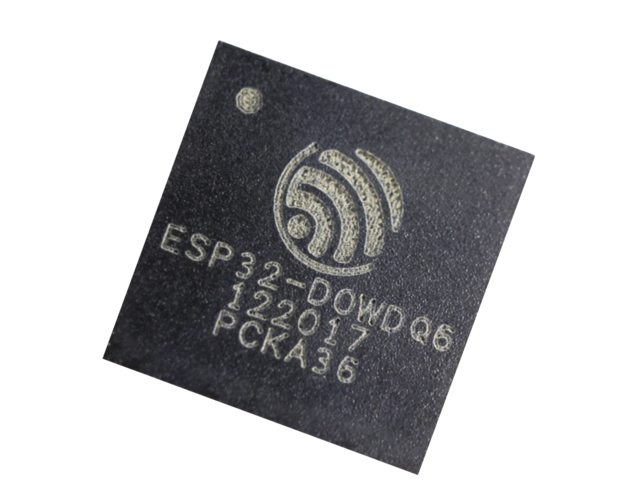
\includegraphics[width=.8\linewidth]{obrazky-figures/esp-soc.png}  
      \caption{SoC}
      %https://www.gridconnect.com/products/esp32-d0wdq6-2-4-ghz-wi-fi-bluetooth-combo-chip
      \label{fig:esp32_soc}
    \end{subfigure}
    \begin{subfigure}{.3\textwidth}
      \centering
      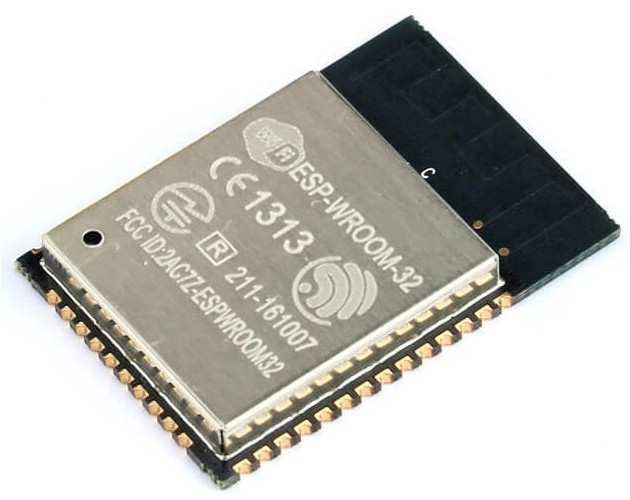
\includegraphics[width=.8\linewidth]{obrazky-figures/esp-module.jpg}  
      \caption{Modul}
      %https://www.blueberrye.me/compute-boards/esp-wroom-32-esp32-wifi-bt-ble-mcu-module/a-1690130
      \label{fig:esp32_module}
    \end{subfigure}
    \begin{subfigure}{.3\textwidth}
      \centering
      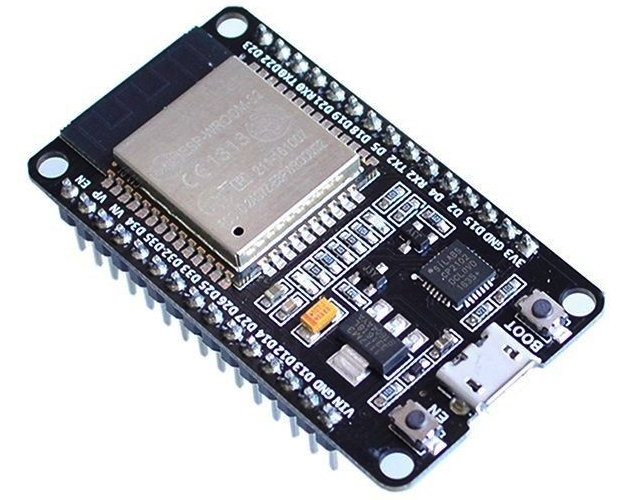
\includegraphics[width=.8\linewidth]{obrazky-figures/esp-dev.png}
      \caption{Vývojová doska}
      %https://navody.arduino-shop.cz/navody-k-produktum/vyvojova-deska-esp32.html
      \label{fig:esp32_dev}
    \end{subfigure}
    \caption{Varianty ESP32}
    \label{fig:esp32_varianty}
\end{figure}


\section{Programovanie}

Existuje viacero možností programovania ESP32. Asi najznámejším a najpoužívanejším je Arduino IDE, prípadne editor s rozšírením PlatformIO. Obe možnosti využívajú pre programovanie jazyk C++. Ide o riešenie s jednoduchou inštaláciou, ktoré ponúka menej možností a väčšie výsledné programy. Na základné aplikácie je často postačujúce. Knižnica je aktualizovaná menej často, čo môže priniesť niekoľko problémov.

Ďalšou z možností je využite frameworku ESP-IDF, ktorý v podstate rieši všetky problémy spomínané v knižnici pre Arduino IDE. Prináša však malú nevýhodu programovania v C a zložitejšiu inštaláciu. Tento nástroj je vyvíjaný samotnou spoločnosťou Espressif Systems a je označovaný za preferovanú formu programovania mikrokontroléru. Je založený na operačnom systéme reálneho času (RTOS), konkrétne na FreeRTOS s otvoreným kódom.

Jedno z možností je aj použitie MicroPython, ktorý je založený na Pythone 3.4 a prináša teda výhody vyššieho programovacieho jazyka. Ide o menej bežný spôsob, a teda existuje na neho menej príkladov a návodov. Zostavenie je založené na frameworku ESP-IDF. Oproti predchádzajúcemu spôsobu ponúka menšie možnosti konfigurácie.

\section{Režim spánku}\label{sec:esp-sleep}

ESP32 podporuje niekoľko režimov spánku čo pomáha ešte viac zmenšovať jeho spotrebu. V tabuľke \ref{tab:spotreba_esp} je možné vidieť porovnanie jednotlivých módov šetrenia energie. V poslednom stĺpci tabuľky sú uvedené len pridané časti, takže pre aktuálny riadok platí to isté čo pre predchádzajúci plus naviac informácie v tomto riadku.

Ako prvý je pre porovnanie uvedený aktívny mód a teda základný mód so všetkými aktívnymi časťami. V prípade súčasného využitia Wi-Fi a Bluetooth môže spotreba dosahovať v špičke až 790~mAh. Pri móde s uspatým modemom (modem sleep) sú neaktívne Wi-Fi, Bluetooth, rádio vysielač a periférie. Je možné nastaviť frekvenciu procesora a upraviť tak spotrebu. V ľahkom spánku (light sleep) je naviac pozastavený procesor, dochádza k uloženiu obsahu RAM. Pri prebudení sa systém vráti do predchádzajúceho stavu. V hlbokom spánku (deep sleep) je procesor úplne vypnutý, koprocesor stále sleduje zmeny na senzoroch a prebúdza procesor. Narozdiel od ľahkého spánku nedochádza k automatickej obnove pamäti RAM. Stále je však možné využiť RTC pamäť na uloženie a znovu načítanie dát pri prebudení. Pri hibernácii (hibernation) je naviac odstavený aj koprocesor a RTC pamäť. Všetko okrem jedného časovača a niektorých vstupných RTC je vypnuté. Tie sú zodpovedné za prebudenie systému.\cite{esp-sleep}

\begin{table}[ht]
    \centering
    \renewcommand{\arraystretch}{1.5}
    \begin{tabular}{|c|c|c|}
        \hline
        Mód & Spotreba & Pridané neaktívne časti \\ \hline
        Active & 80-260 mA\footnotemark & - \\ \hline
        Modem sleep & 3-20 mA & Wi-Fi, Bluetooth, periférie, vysielač\\ \hline
        Light sleep & 0,8 mA & pozastavený procesor\\ \hline
        Deep sleep & 10 $\mu$A & procesor\\ \hline
        Hibernation & 2.5 $\mu$A & koprocesor\\ \hline
    \end{tabular}
    \caption{Porovnanie spotreby v jednotlivých módoch\cite{esp-sleep}}
    \label{tab:spotreba_esp}
\end{table}
\footnotetext{V prípade zasielania dát pomocou Wi-Fi alebo Bluetooth je spotreba vyššia ako pri prijímaní}

\chapter{Návrh prototypu}

Cieľom práce je navrhnúť zabezpečovacie zariadenie, ktoré bude schopné detekovať prítomnosť majiteľa pomocou BLE. Výsledné zariadenie musí obsahovať BLE modul, pomocou ktorého bude pravidelne skenovať okolie pre prítomnosť známych zariadení. O skenovanie sa pritom bude starať samotná ústredňa zabezpečovacieho zariadenia, ktorá zároveň vyhodnocuje informácie zo senzorov. Na základe toho sa systém dokáže prepínať medzi rôznymi stavmi (odstrážené, zabezpečené, alarm a podobne).

Celý navrhovaný systém môžeme vidieť ako blokový diagram na obrázku \ref{fig:navrh_diagram}. Súčasťou diagramu sú obe časti systému - ústredňa aj samotné senzory. Podrobnejšie sa k jednotlivým častiam venujem v nasledujúcich kapitolách.

\begin{figure}[ht]
    \centering
    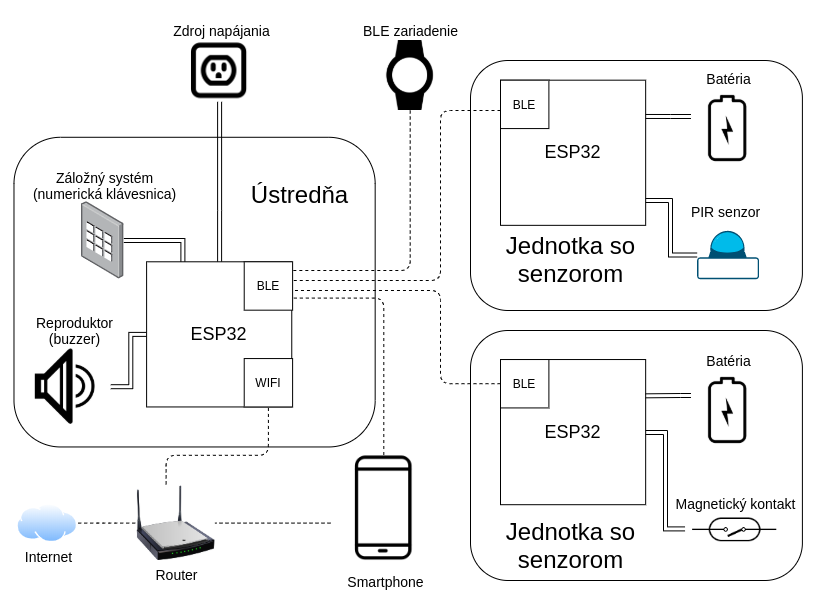
\includegraphics[scale=0.4]{obrazky-figures/block_diagram.png}
    \caption{Blokový diagram prototypu}
    \label{fig:navrh_diagram}
\end{figure}

\section{Stavy systému}

Prototyp by mal byť schopný rozlišovať rôzne stavy stráženia a prepínať medzi nimi. Na obrázku \ref{fig:state_diagram} je zobrazený stavový diagram, ktorý ukazuje jednotlivé stavy a prechody medzi nimi.

\begin{figure}[ht]
    \centering
    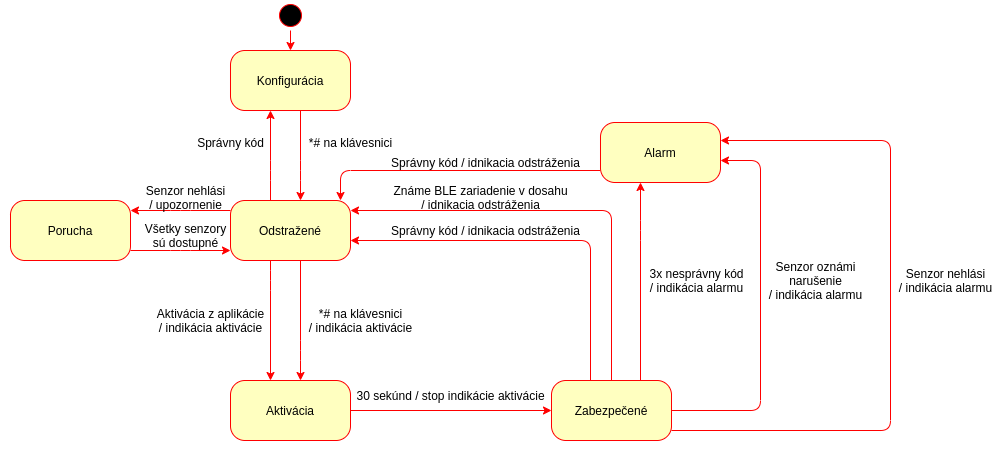
\includegraphics[scale=0.5]{obrazky-figures/state_diagram.png}
    \caption{Stavový diagram prototypu}
    \label{fig:state_diagram}
\end{figure}

Navrhované stavy zahrňujú:

\begin{itemize}
    \item \textbf{konfigurácia} - stav určený pre konfiguráciu samotného systému. V tomto stave je možné zmeniť kód, ktorým sa zariadenia dokáže prepnúť zo stavu zabezpečené naspäť do stavu odstrážené. Zároveň je možné zmeniť známe zariadenia, nastavenia Wi-Fi siete a podobne. 
    \item \textbf{odstrážené} - režim, v ktorom je systém pripravený kedykoľvek na prepnutie do stavu aktivácie systému. V tomto režime sa kontrolujú pripojené senzory, nie však ich výstup, ale len ich dostupnosť.
    \item \textbf{aktivácia} - prechodový stav trvajúci niekoľko sekúnd. Počas aktivácie systému ústredňa vydáva signalizáciu o tom, že je čo najskôr nutné opustiť strážené priestory. Zároveň ústredňa oznámi senzorom tento stav a tie sa presunú do stavu zabezpečené.
    \item \textbf{zabezpečené} - po aktivácii sa systém automaticky prepne do stavu strážené. V tomto stave sa vyhodnocujú prijaté informácie z jednotlivých senzorov a v prípade, že je zaznamenané narušenie zmení sa stav na alarm. Zároveň v tomto režime opakovane prebieha aktívny sken okolia pre známe BLE zariadenia. V prípade, že sa takéto zariadenia nájde a ústredňa je schopná sa k nemu pripojiť, vykoná sa deaktivácia systému a teda zmena stavu na odstrážené. Druhým spôsobom prechodu do stavu odstrážené je zadaním správneho kódu na číselnej klávesnici. V prípade opakovaného zadania nesprávneho kódu prejde systém do stavu alarm.
    \item \textbf{alarm} - nastane v prípade zaznamenania neoprávneného vstupu do objektu. Ústredňa spustí indikáciu alarmu. Z tohto stavu dá dostať jedine zadaním správneho kódu na číselnej klávesnici. Následne je systém uvedený do stavu odstrážené a je pripravený na ďalšie použitie.
\end{itemize}

Všetky spomínané stavy platia pre ústredňu systému. Pre jednotky so senzormi stačí pre jednoduchosť uvažovať len nad stavom stráženia a pohotovostných režimom. Tento režim môže chápať aj ako stav odstrážené, kedy senzory ústredni len oznamujú, že nedošlo k žiadnej chybe, sú stále dostupné, teda overujeme integritu spojenia.

\section{Ústredňa}

Ústredňu v tomto prípade tvorí vývojový modul s mikrokontrolérom ESP32. Ten je vhodný hlavne vďaka jeho dostupnosti a podpore všetkých potrebných technológií. Na modul sú následne pripojené jednotlivé signalizačné zariadenia ako je reproduktor (bzučiak) alebo ďalšie LED diódy a podobne. Tieto zariadenia informujú prevažne o zmenách stavu systému ako je napríklad prepínanie do módu stráženia. To je dôležité ako upozornenie pre majiteľa, že systém sa aktivuje, a teda by mal opustiť strážený priestor. V navrhovanom systéme je to hlavne dôležité, aby sa majiteľ dostal z dosahu hlavnej jednotky so svojím Bluetooth zariadením, inak by systém mohol nechcene prepnúť do režimu odstrážené.

Pre napájanie systému je navrhnuté priame napájanie z elektrickej siete. To je potrebné hlavne z dôvodu súčasného využívania Wi-Fi a Bluetooth technológií, ktoré sú najviac náročné na spotrebu, ako bolo spomenuté v kapitole \ref{sec:esp-sleep}. Prípadne napájanie je vhodné realizovať pomocou kombinácie napájanie z elektrickej siete a batériou. V tomto prípade by sa primárne preferovala elektrická sieť, pri jej prípadnom výpadku by sa plynulo prešlo na záložnú batériu.

\subsection{Pripojené zariadenia}

Ústredňa sa okrem ESP32 skladá aj z ďalších zariadení, ktoré pomáhajú indikovať stavy systému, prípadne nejaký záložný systém v prípade vybitia BLE zariadenia, strata, odcudzenie a podobne. Týmto záložným systémom môže byť napríklad kódová klávesnica. Tá je vhodná hlavne vďaka jednoduchosti na použitie, zároveň so sebou nie je nutné nič nosiť, stačí si zapamätať kód.

K indikačným zariadeniam môžme zaradiť LED diódy, reproduktor alebo bzučiak. Tieto zariadenia indikujú stav systému, prípadne zmenu stavu. Ústredňa by mala obsahovať minimálne jednu LED diódu, na indikáciu upozornenia a druhá dióda by mala slúžiť ako indikácia narušenia. V prípade aktivácie zabezpečenia systém opakovane bliká upozorňovacou diódou a vydáva tón, aby oznámil majiteľovi, že má opustiť priestor. V prípade alarmu sa aktivuje indikácia narušenia spolu s zvukový oznámením. Pri deaktivácii systému rozsvieti sa indikácia upozornenia a zároveň krátkym tónom sa ohlási zmena stavu na odstrážené.

\subsection{Komunikácia so zariadeniami}

Okrem iného sa ústredňa stará o komunikáciu s uloženými zariadeniami. Pre nastavenie nového zariadenia sa ústredňa pokúsi na takéto zariadenia pripojiť pomocou tzv. \texttt{bondingu}. Je vyžadované aby zariadenie podporovalo šifrovanú komunikáciu pomocou BLE. V prípade, že to zariadenie nepodporuje nie je možné ho pridať na zoznam známych zariadení, a teda deaktivovať EZS pomocou neho. Šifrovanie je vyžadované hlavne kvôli bezpečnosti, keďže je jednoduché skopírovať zariadenie.

\subsection{Štruktúra BLE služieb}\label{sec:BLE_struc}

Ústredňa obsahuje 3 BLE služby. Tie sú rozdelené podľa ich funkcie na:
\begin{itemize}
    \item \textbf{služba stavu systému} - pomocou tejto služby senzory zisťujú stav systému a podľa neho upravujú svoje nastavenie. Zároveň slúži aj ako overenie, že senzor je dostupný a teda prečítal charakteristiku.
    \item \textbf{služba alarmu} - slúži na zápis oznámenia o narušení. Senzor zapíše nenulovú hodnotu v prípade, že zaznamenal narušenie.
    \item \textbf{služba nastavenia systému} - využíva sa na počiatočné nastavenie systému. Slúži na komunikáciu s mobilným zariadením. Aplikácia odošle meno a heslo pre Wi-Fi sieť. Pri prečítaní systém vráti IP adresu ústredne.
\end{itemize}

Každá služba obsahuje práve jednu charakteristiku, vlastné unikátne identifikačné číslo. Konkrétny prehľad usporiadania služieb spolu s povolenými metódami je graficky znázornený na obrázku \ref{fig:BLE_structure}.

\begin{figure}[ht]
    \centering
    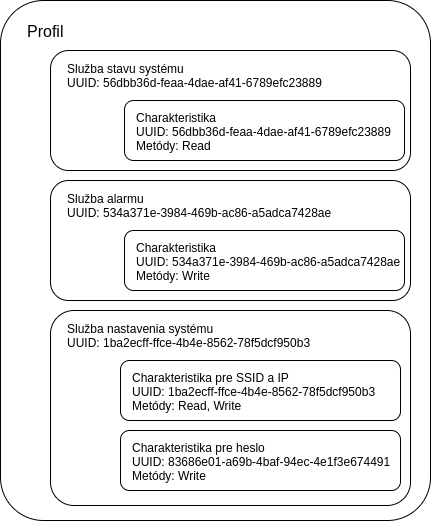
\includegraphics[scale=0.5]{obrazky-figures/BLE_structure.png}
    \caption{Štruktúra BLE služieb}
    \label{fig:BLE_structure}
\end{figure}

\section{Jednotka so senzorom}

Hlavnou časťou jednotky so senzorom je ESP32, ktoré pomocou BLE komunikuje s ústredňou. Konkrétne spôsob komunikácie je popísaný v kapitole \ref{sec:komunikacia}. Okrem ESP je súčasťou jednotky aj samotný senzor a indikačná LED dióda. Tá sa rozsvieti v prípade, že je systém v stave zabezpečené a bolo zaznamenané narušenie priestoru. Táto jednotka by mala podporovať minimálne PIR senzor a magnetický senzor. Všeobecne by však zariadenie malo podporovať akýkoľvek senzor, ktorý pri zistení narušenia dá na výstup napätie na úrovni logickej 1 prípadne 0.

\subsection{Použité senzory}

Medzi použité senzory boli zaradené najdostupnejšie senzory. Zároveň bol dávaný dôraz aj na ich spotrebu. Senzory by pri tom mali byť schopné pri narušení oznámiť túto skutočnosť jednoduchým zmenením svojho výstupu na opačnú hodnotu.



\subsection{Napájanie}

Napájanie jednotky so senzorom by malo byť realizované pomocou batérie. Tým by sa mal systém stať jednoduchším na inštaláciu a prípadne zmeny umiestnenia jednotlivých senzorov. Je však nutné aby takéto napájanie vydržalo aspoň rok. Pri výpočte vhodnej kapacity musíme počítať so spotrebou ESP32 ako aj so spotrebou samotného senzoru. Môžme pritom uvažovať niekoľko stavov:
\begin{itemize}
    \item systém je stále v stave \textit{odstrážené}. Zariadenie je v stave hlbokého spánku dlhšiu dobu.
    \item systém pravidelne strieda stavy. Ide o očakávané zaobchádzanie so systémom. Počíta s tým, že s tým že systém je rovnaký čas v oboch stavoch.
    \item systém je stále v stave \textit{zabezpečené}. Ide o extrém, kde je systém stále aktivovaný, teda hlboký spánok je obmedzený na kratšiu dobu. V tomto prípade je spotreba energie najvyššia.
\end{itemize}

Týmto rozdelením môžme získať minimálnu, priemernú a maximálnu spotrebu systému. 

TODO: výpočet spotreby

\section{Komunikácia ústredne so senzormi}\label{sec:komunikacia}

Pri komunikácií so senzormi sa využíva technológia BLE. Ústredňa vystupuje ako server, na ktorý sa pripájajú senzory ako klienti. V kapitole \ref{sec:BLE_struc} je opísaná štruktúra serveru. Klient sa najprv pripojí na server, následne zistí stav ústredne prečítaním hodnoty služby. Následne podľa zisteného stavu urobí jedno z:
\begin{itemize}
    \item ak je systém v stave konfigurácie alebo odstrážené, jednotka so senzorom sa uspí na 40 sekúnd. Senzor je v tomto prípade deaktivovaný. Tento spôsob je vhodný hlavne pre šetrenie batérie jednotky.
    \item v ostatných stavoch sa jednotka so senzorom uspí na 20 sekúnd. Zároveň sa aktivuje prebudenie jednotky pomocou senzora. V prípade prebudenia zo senzora sa na príslušnú službu serveru zapíše oznámenie o narušení.
\end{itemize}
Po oboch variantách sa jednotka so senzorom uspí na stanovený čas. Následne znova oznámi svoju funkčnosť ústredni a zistí stav systému. Rozhodovanie sa opakuje.

\section{Správa systému}

Celý systém je potrebné spravovať. Keďže samotný systém neobsahuje žiadnu zobrazovaciu jednotku, ako je displej, nie je možné túto správu vykonávať priamo z ústredne. Túto funkciu v navrhovanom systéme bude zastrešovať mobilná aplikácia. Tá by sa mala postarať o nasledovné funkcie:
\begin{itemize}
    \item \textbf{počiatočné nastavenie systému} - slúži na nastavenie názvu a hesla Wi-Fi siete, na ktorú sa má zariadenie pripojiť. Následne sa odošle odpoveď z ústredne v podobe IP adresy ústredne.
    \item \textbf{zmena číselného kódu} - zmena aktuálneho kódu, ktorý slúži na deaktiváciu systému a prepnutie do stavu konfigurácie.
    \item \textbf{správa senzorov} - zobrazenie základných informácií o senzore, pridávanie nových senzorov, prípadne ich odoberanie.
    \item \textbf{správa spárovaných zariadení} - pridávanie nových zariadení, odstraňovanie zariadení. Slúžia na automatickú deaktiváciu systému.
    \item \textbf{aktivácia systému} - aktivácia systému pomocou aplikácie, teda prepnutie do stavu aktivácie a následne do stavu zabezpečené.
\end{itemize}

Odosielanie takmer všetkých požiadaviek na ústredňu bude prebiehať pomocou HTTP na lokálnej sieti. Je teda nutné aby obe zariadenia boli pripojené na rovnakú Wi-Fi sieť. Výnimkou budú počiatočné nastavenia, ktoré slúžia práve na nastavenie komunikácie pomocou Wi-Fi. Tieto počiatočné nastavenia budú prebiehať pomocou technológie BLE. Pri všetkých nastaveniach musí byť systém v stave konfigurácie, jedinou výnimkou je aktivácia systému, ktorá okrem stavu konfigurácie podporuje aj stav odstrážené.

\chapter{Implementácia}

\section{ESP32}

\subsection{Ústredňa}

\subsection{Jednotka so senzorom}

\section{Mobilná aplikácia}

\section{Nastavenie systému}



\chapter{Vlastnosti systému a možné rozšírenia}

\section{Vlastnosti systému}

\section{Rozšírenia}

